\chapter{构建黑洞与近视界之谜}

\lectureoverview{我们将用三块材料来构建一个黑洞：平直时空的因果图、施瓦西图，以及球壳的伯克霍夫定理。这一构建表明，事件视界是一个整体边界，并且可以起始于一个局部仍然平直的区域。随后我们从因果几何转向熵与霍金温度。置于视界附近的温度计会变得任意热，而自由下落的观测者却预期不会发生局部灾难。最后的论证追问：外部实验在不制造它本应探测的扰动的前提下，究竟能确立什么。}

\section{处于空空间温度下的黑洞}

本来应该有一份作业：构建一个黑洞并把它带到课堂上展示讲解。没有人有黑洞可以展示，但通过 Wolfram 找到的一个计算提供了一个更温和的开场问题。什么样的半径和质量会使一个黑洞的霍金温度接近宇宙微波背景的 \(3\,\mathrm{K}\) 温度？

\begin{classroomqa}
\audiencequestion{网站上计算了什么？\lecturetimestamp{00:00:39}}
\lecturerresponse{一个温度约为 \(3\,\mathrm{K}\) 的黑洞的半径。重点不在于精确计算，而在于对物理尺度的估计。}
\end{classroomqa}

这样的黑洞会暂时与其周围环境具有相同的温度，但这种平衡是不稳定的。施瓦西黑洞具有负热容。如果它变得比热浴稍热，它就会辐射，失去质量，并变得更热。如果它变得稍冷，它就会吸收，获得质量，并变得更冷。\editorialnote{这就是课堂上故意宽松的措辞背后精确的稳定性论证。正则热浴无法为孤立的施瓦西黑洞提供稳定的平衡。}

估计从 \(3\,\mathrm{K}\) 辐射的特征波长开始。

\begin{classroomqa}
\audiencequestion{约三开尔文的辐射对应什么波长？\lecturetimestamp{00:02:03}}
\lecturerresponse{教室里有人提出一厘米、\(21\) 厘米，甚至 \(10\) 米，最后才确定在微波波段。对于论证有用的数量级答案约为一厘米，小到足以开微波炉和面包盒的玩笑。}
\end{classroomqa}

典型的霍金量子的波长与施瓦西半径相当，相差数值因子：
\begin{equation}
\lambda_{\mathrm{H}}\sim R_s,
\qquad
R_s=\frac{2GM}{c^2}.
\label{eq:l05-scale}
\end{equation}
取课堂值 \(\lambda_{\mathrm H}\sim1\,\mathrm{cm}\) 得到 \(R_s\sim1\,\mathrm{cm}\)。由于一个太阳质量的黑洞半径只有几公里，而 \(R_s\) 正比于 \(M\)，相应的质量大致为
\begin{equation}
M\sim10^{-5}M_\odot,
\label{eq:l05-rough-mass}
\end{equation}
这属于行星尺度。这就是为什么讲座得出一个类似地球的估计。

\begin{classroomqa}
\audiencequestion{这与 Wolfram 的数值结果一致吗？\lecturetimestamp{00:05:53}}
\lecturerresponse{报告的结果更接近月球的质量。与粗略估计相比这听起来很小，但无论哪个答案都说明了预期的要点：这个物体不是能装进口袋的东西。}
\end{classroomqa}

保留常数可以解释这一差异。由
\begin{equation}
T_H=\frac{\hbar c}{4\pi k_B R_s},
\end{equation}
在 \(T_H=3\,\mathrm{K}\) 时可得，
\begin{equation}
R_s\simeq6.1\times10^{-5}\,\mathrm{m},
\qquad
M\simeq4.1\times10^{22}\,\mathrm{kg}.
\label{eq:l05-three-kelvin}
\end{equation}
这是月球而非地球的质量。微波波长、因子 \(4\pi\)，以及选择哪个黑体波长作为典型值，共同造成了快速估计与数值之间的差距。\editorialnote{方程~\eqref{eq:l05-three-kelvin}恢复了讲座在量纲估计中省略的数值因子。估计本身被保留，因为它是课堂上使用的路径。}

算术已经完成了它的使命。我们现在想要在数学上和想象中构建一个黑洞。完整的场方程对于当前目的来说太难了。图像将提供基本事实。

\section{第一个工作部件：平直时空}

使用以观测者为中心的极坐标并抑制角度。约化坐标为 \((t,r)\)，其中 \(r\geq0\)。这个约化图中的一个点不是四维时空中的一个点；除 \(r=0\) 外，它代表整个二维球面 \(S^2\)。

径向光线以 \(45^\circ\) 运动。入射光线到达原点，出射光线沿另一零方向离开原点。通过共形变换，无限半平面可以被压缩成有限的彭罗斯楔形。该变换不是唯一的。其本质性质是无穷远被带到有限边界，并且径向零方向保持在 \(45^\circ\)。用黑板上的话说，我们把图压扁了。

\begin{figure}[htbp]
\centering
\includegraphics[width=0.68\textwidth]{lecture_05_figure_02.png}
\caption{紧致化径向闵可夫斯基时空的上半部分。竖直边为\(r=0\)，而曲线族向紧致化无穷远处聚集。}
\lectureframe{00:11:41.560}
\end{figure}

\begin{figure}[htbp]
\centering
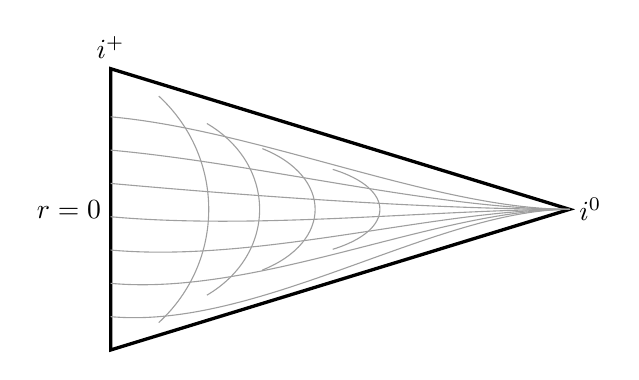
\begin{tikzpicture}[scale=0.94]
\coordinate (O) at (0,0);
\coordinate (P) at (0,3.8);
\coordinate (I) at (6.2,1.9);
\draw[very thick] (O)--(P)--(I)--cycle;
\foreach \y in {0.45,0.90,1.35,1.80,2.25,2.70,3.15} {
  \draw[gray!75] (0,\y) .. controls (2.0,\y-0.18) and (4.4,1.9) .. (I);
}
\draw[gray!75] (0.65,0.37) .. controls (1.55,1.20) and (1.55,2.60) .. (0.65,3.43);
\draw[gray!75] (1.30,0.74) .. controls (2.25,1.30) and (2.25,2.50) .. (1.30,3.06);
\draw[gray!75] (2.05,1.08) .. controls (3.00,1.46) and (3.00,2.34) .. (2.05,2.72);
\draw[gray!75] (3.00,1.36) .. controls (3.85,1.62) and (3.85,2.18) .. (3.00,2.44);
\node[left] at (0,1.9) {\(r=0\)};
\node[above] at (P) {\(i^+\)};
\node[right] at (I) {\(i^0\)};
\end{tikzpicture}
\caption{上半楔形区域的清晰版本。这些曲线是定性的等\(r\)线和等\(t\)线族，并非精确的坐标网格。}
\label{fig:l05-flat-wedge}
\end{figure}

固定\(r\)的世界线在紧致化前是竖直的，随后弯曲并在未来类时无穷远附近聚集。等\(t\)切片同样向空间无穷远聚集。这种聚集是坐标效应，而非物质的物理压缩。

\(45^\circ\)规则直接适用于径向光。具有角动量的光线可能不经过原点，而是到达一个非零的最近距离后向外返回。远离原点时，其投影运动看起来几乎是径向的；只有在最近距离附近，约化的\((t,r)\)轨迹才明显弯曲。至此，第一部分工作完成。

\section{第二部分工作：永恒施瓦茨席尔德}

最大延拓的施瓦茨席尔德解有两个外部菱形区域、一个未来黑洞区域和一个过去白洞区域。其上、下波浪形边界分别是未来奇点和过去奇点。对于由坍缩形成的黑洞，这一结构的大部分很快就会被丢弃，但普通的右侧外部区域正是我们所需的部分。

\begin{figure}[htbp]
\centering
\includegraphics[width=0.72\textwidth]{lecture_05_figure_03.png}
\caption{永恒施瓦茨席尔德图，右侧为普通外部区域及其示意性坐标网格。}
\lectureframe{00:16:55.975}
\end{figure}

\begin{figure}[htbp]
\centering
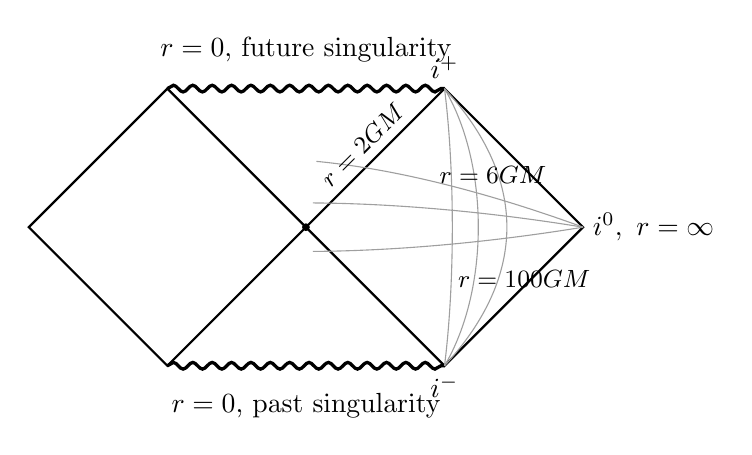
\begin{tikzpicture}[scale=0.88]
\coordinate (C) at (0,0);
\coordinate (TL) at (-2.0,2.0);
\coordinate (L) at (-4.0,0);
\coordinate (BL) at (-2.0,-2.0);
\coordinate (TR) at (2.0,2.0);
\coordinate (R) at (4.0,0);
\coordinate (BR) at (2.0,-2.0);
\draw[thick] (C)--(TL)--(L)--(BL)--(C);
\draw[thick] (C)--(TR)--(R)--(BR)--(C);
\draw[very thick,decorate,decoration={snake,amplitude=1.2pt,segment length=7pt}] (TL)--(TR);
\draw[very thick,decorate,decoration={snake,amplitude=1.2pt,segment length=7pt}] (BL)--(BR);
\draw[gray!75] (TR) .. controls (2.15,0.8) and (2.15,-0.8) .. (BR);
\draw[gray!75] (TR) .. controls (2.65,0.9) and (2.65,-0.9) .. (BR);
\draw[gray!75] (TR) .. controls (3.20,0.7) and (3.20,-0.7) .. (BR);
\draw[gray!75] (0.15,0.95) .. controls (1.5,0.82) and (2.9,0.40) .. (R);
\draw[gray!75] (0.10,0.35) .. controls (1.5,0.34) and (2.9,0.18) .. (R);
\draw[gray!75] (0.10,-0.35) .. controls (1.5,-0.34) and (2.9,-0.18) .. (R);
\fill (C) circle (1.6pt);
\node[above] at (TR) {\(i^+\)};
\node[below] at (BR) {\(i^-\)};
\node[right] at (R) {\(i^0,\ r=\infty\)};
\node[above] at (0,2.25) {\(r=0\), future singularity};
\node[below] at (0,-2.25) {\(r=0\), past singularity};
\node[rotate=45,above,font=\small] at (1.0,1.0) {\(r=2GM\)};
\node[font=\small] at (2.70,0.75) {\(r=6GM\)};
\node[font=\small] at (3.15,-0.75) {\(r=100GM\)};
\end{tikzpicture}
\caption{右侧外部区域在大半径处类似于平坦楔形。当\(c=1\)时，其内部零边为\(r=2GM\)；其他标注的半径是示意性示例。}
\label{fig:l05-eternal-schwarzschild}
\end{figure}

远离黑洞处，外部区域越来越像紧致化的平坦空间。诸如\(r=6GM\)和\(r=100GM\)这样的线趋近于普通等半径世界线的行为。外部区域的内边界位于
\begin{equation}
r=2GM
\end{equation}
单位为\(c=1\)。

在中心附近，与平坦空间的比较失效。闵可夫斯基空间中的径向光线到达\(r=0\)后从相反的物理侧重新出现。施瓦茨席尔德内部指向未来的光线不会反弹。它终止于\(r=0\)处的类空奇点。这一因果差异正是坍缩构造必须保持的。

\section{让我们把各部分拼接起来的定理}

缺失的要素首先出现在牛顿引力中。对于球对称质量分布，高斯定律给出
\begin{equation}
\oint\mathbf g\cdot d\mathbf A=-4\pi G M_{\mathrm{enc}},
\end{equation}
因此
\begin{equation}
\mathbf g(r)=-\frac{G M_{\mathrm{enc}}(r)}{r^2}\,\hat{\mathbf r}.
\label{eq:l05-shell-theorem}
\end{equation}
半径\(r\)的球面之外的物质对该处不贡献净场。对于总质量为\(M\)的空心球壳，
\begin{equation}
\mathbf g=
\begin{cases}
0, & r<R_{\mathrm{shell}},\\[3pt]
-\dfrac{GM}{r^2}\hat{\mathbf r}, & r>R_{\mathrm{shell}}.
\end{cases}
\end{equation}

伯克霍夫定理是相对论性的替代。每个球对称真空区域局部上都是具有恒定质量参数的施瓦茨席尔德区域。球形壳层的空内部质量参数为零，局部上是闵可夫斯基的；外部质量参数为\(M\)，是施瓦茨席尔德的：
\begin{equation}
\begin{aligned}
M_{\mathrm{enc}}&=0 && \text{inside the shell},\\
M_{\mathrm{enc}}&=M && \text{outside the shell}.
\end{aligned}
\label{eq:l05-birkhoff}
\end{equation}
当壳层运动时，该陈述仍然有用，因为两侧的真空区域保持球对称。

\editorialnote{内部平坦是一个局部陈述。即使内部曲率消失，静态壳层也可以改变内部时间坐标的归一化。对于运动或零壳层，两个真空度规必须在壳层处匹配；理想化构造是薄壳连接，与入射Vaidya几何密切相关。这些限定条件都不改变此处使用的因果剪贴论证。}

对于实验室图像，想象一个球面密布着同步激光器，如同大型惯性约束装置中那样，全部同时向内发射。在理想化中不存在仪器，只有一个完美球形的光壳层。壳层携带能量\(E\)，因此外部质量参数为
\begin{equation}
M=\frac{E}{c^2},
\end{equation}
或在自然单位下简写为\(E=M\)。由于壳层以光速运动，它在约化图上是一条入射零线。该线上的每个点代表整个球面波前，而非单个光子轨迹。

\section{缝合坍缩时空}

从平坦时空开始，画出入射零壳层。壳层内部是正确的：伯克霍夫定理表明它是平坦的。壳层外部是错误的，因为外部必须已经通过其施瓦茨席尔德几何知道壳层的总质量。

现在在永恒施瓦茨席尔德图中画出同一个壳层。在那里，壳层外部的区域是正确的。对于从普通真空中开始的坍缩而言，白洞、第二个外部区域以及黑洞内部不适当的部分都是错误的，因此把它们擦掉。

\begin{figure}[htbp]
\centering
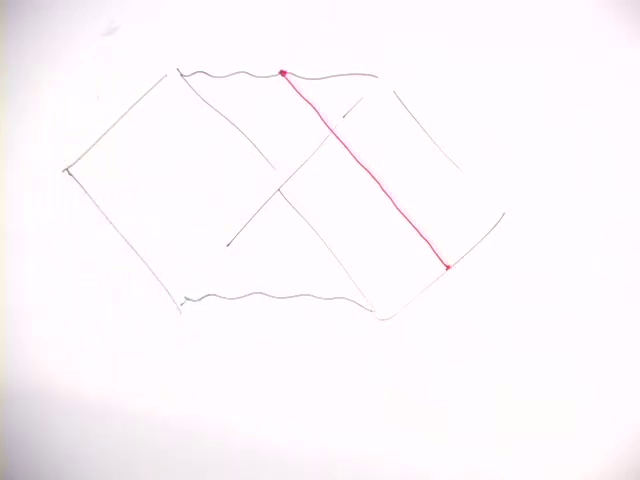
\includegraphics[width=0.72\textwidth]{lecture_05_figure_05.png}
\caption{零质量壳层，以红色表示，画在施瓦茨席尔德图上，同时正确的部分被分离出来。}
\lectureframe{00:32:00.000}
\end{figure}

壳层在平坦部分到达\(r=0\)。在施瓦茨席尔德部分，它到达未来奇点的起点。这两个是同一个端点。沿壳层把平坦内部与施瓦茨席尔德外部粘合起来，就得到黑洞形成的最简单时空。

\begin{classroomqa}
\audiencequestion{在左上方的连接点处，平坦空间的端点真的与施瓦茨席尔德一侧的点相同吗？\lecturetimestamp{00:34:50}}
\lecturerresponse{是的。平坦空间中的壳层收缩到\(r=0\)，而施瓦茨席尔德奇点也在\(r=0\)。被等同起来的这两个点具有相同的几何意义：二维球面已经收缩到零尺度。}
\end{classroomqa}

\begin{figure}[htbp]
\centering
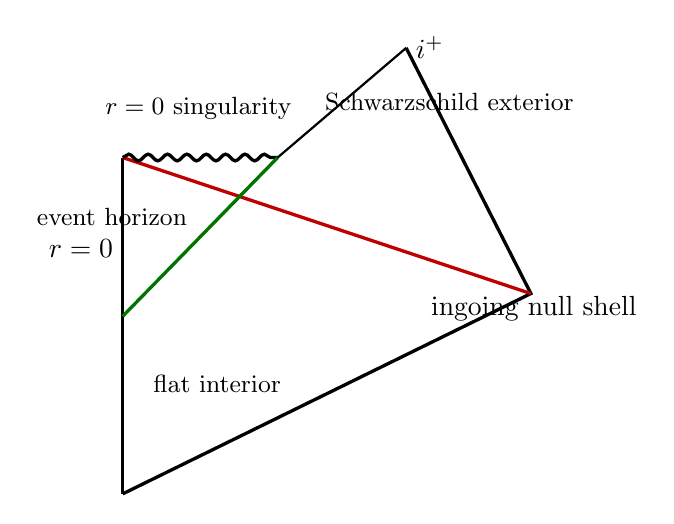
\begin{tikzpicture}[scale=0.96]
\coordinate (A) at (0,-2.8);
\coordinate (B) at (0,1.65);
\coordinate (C) at (2.05,1.65);
\coordinate (D) at (5.4,-0.15);
\coordinate (E) at (3.75,3.10);
\coordinate (H0) at (0,-0.45);
\draw[very thick] (A)--(B);
\draw[very thick] (A)--(D)--(E);
\draw[very thick,red!75!black] (D)--(B);
\draw[very thick,decorate,decoration={snake,amplitude=1.2pt,segment length=7pt}] (B)--(C);
\draw[very thick,green!45!black] (H0)--(C);
\draw[thick] (C)--(E);
\node[left] at (0,0.45) {\(r=0\)};
\node[below right] at (3.95,-0.05) {ingoing null shell};
\node[font=\small] at (1.25,-1.35) {flat interior};
\node[font=\small,anchor=west] at (2.55,2.38) {Schwarzschild exterior};
\node[above,font=\small] at (1.0,2.02) {\(r=0\) singularity};
\node[above left,font=\small] at (0.98,0.62) {event horizon};
\node[right] at (E) {\(i^+\)};
\end{tikzpicture}
\caption{坍缩几何。红色壳层把平坦内部与施瓦茨席尔德外部连接起来。绿色事件视界在平坦区域中开始得更早，并终止于黑洞区域的未来边界。}
\label{fig:l05-collapse}
\end{figure}

这一构造回答了永恒解所遗留的一个问题。由坍缩形成的黑洞没有过去的白洞，也没有第二个渐近宇宙。它仍然有一个未来奇点。

\section{视界是一个整体边界}

旧的标签\(r=2GM\)在静态施瓦茨席尔德几何中标识了视界，但它并不是动力学时空中所需的定义。

\begin{definition}
未来事件视界是能够向未来零无穷发送未来指向因果信号的事件集合的边界。
\end{definition}

在坍缩图上，追踪那条恰好无法逃逸的向外零射线。紧靠它外侧的射线到达无穷远；紧靠它内侧的射线终止于奇点。那个分隔者就是真正的视界。

\begin{figure}[htbp]
\centering
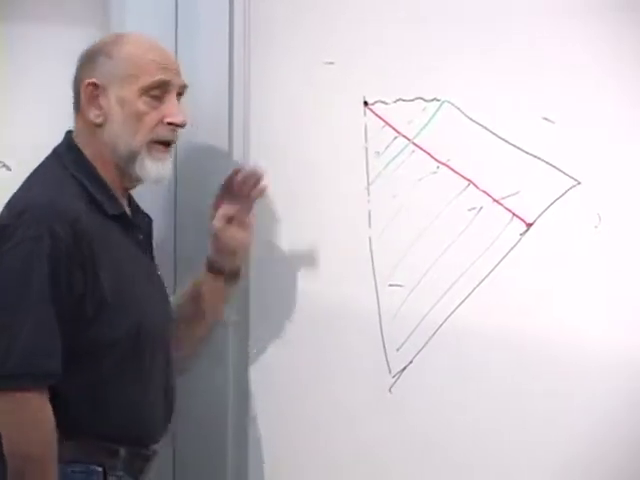
\includegraphics[width=0.72\textwidth]{lecture_05_figure_06.png}
\caption{完成的黑板构造。入射壳层为红色，事件视界为绿色；绿线的一部分位于壳层下方仍为平坦的区域中。}
\lectureframe{00:39:10.000}
\end{figure}

令人惊讶的特征现在不可避免。视界向后延伸到壳层尚未到达的区域。那里的几何局部是平坦的，穿过那条线的观测者不会探测到曲率脉冲、墙或闪光。然而，该观测者已经无法到达无穷远，因为未来的壳层将封闭所有可能的逃逸路径。事件视界正是在这种整体意义上具有目的论性质：定位一个事件视界需要知道时空的整个未来。\editorialnote{没有任何局部实验能够确定一个光滑的事件视界刚刚被穿过。其他概念，例如表观视界或捕获视界，更为局部，并且在坍缩过程中不必与事件视界重合。}

排水口类比隔离出了因果观念。想象一个划船者位于静止湖中一个被塞住的排水口附近。如果塞子永远不拔，划船者可以离开。如果某人必定会拔掉它，那么即使水尚未流动，后来的水流也可能使逃逸变得不可能。冻结的尼亚加拉瀑布说明了同一点：平静的水并不保证未来有通往安全的路线。

\begin{classroomqa}
\audiencequestion{塞子被拔掉是因为光的球面壳层变得越来越集中吗？\lecturetimestamp{00:43:13}}
\lecturerresponse{这种集中创造了黑洞，但排水口故事被用于一个更狭窄的目的：在局部发生任何戏剧性事件之前，一个人可能已经越过了不可返回点。}
\end{classroomqa}

\subsection{由增长球面构成的视界}

约化视界上的每一点都代表一个\(S^2\)。在视界的第一个点处，该球面面积为零。沿视界向上移动，球面不断增长，直到其面积半径达到
\begin{equation}
R_s=\frac{2GM}{c^2}.
\end{equation}
对于静态黑洞，它保持该尺度；如果有更多能量落入，它会再次增长。

\editorialnote{在理想化球对称坍缩图中，视界生成元在\(r=0\)上的一个形成点或折痕处相交。正是这个极限二维球面具有零面积；不应把该陈述理解为有限的施瓦茨席尔德视界突然收缩到一个点。}

\subsection{遥远观测者能够重构什么}

接下来的长篇讨论把已经处于整体视界内部的观测者与该观测者如何到达那里的历史区分开来。

\begin{classroomqa}
\audiencequestion{在壳层到达之前，被困者的状态是什么？从远处观察者的角度来看，那个人是否在视界之外？\lecturetimestamp{00:44:03}}
\lecturerresponse{不。一旦世界线位于事件视界之后，它的未来就到达奇点，并且它发出的任何新信号都无法到达远处观察者。然而，那个人并非在那里开始存在。更早的粒子、祖先或其他前驱能量是从一个可见区域进入的。}
\end{classroomqa}

因此，远处观察者可能看到前驱物质接近视界，却从未接收到来自视界之外的信号。看穿入射壳层并无矛盾：它由光构成，观察者也能看到壳层本身，并推断黑洞已经形成。

\begin{classroomqa}
\audiencequestion{视线是否穿过坍缩壳层，外部观察者是否仍能知道黑洞已经形成？\lecturetimestamp{00:46:51}}
\lecturerresponse{是的。观察者看到入射壳层，并且能够接收到其路径穿过该壳层的光，只要那光仍能逃逸。看起来奇怪的是，前驱物质甚至在壳层到达中心之前就接近了新确定的视界。}
\end{classroomqa}

\begin{classroomqa}
\audiencequestion{这是否延续了那条规则：从外部看，物质看起来像是被压缩到了视界上？\lecturetimestamp{00:47:49}}
\lecturerresponse{是的。在外部描述中，它仍然与视界相关联，红移越来越大，直到后来黑洞蒸发的量子过程改变了这一图景。}
\end{classroomqa}

这种外部描述引出了下一个主题。如果信息看起来被涂抹在一个二维表面上，那么黑洞熵与该表面面积成正比就不那么令人惊讶了。

\section{从无穷远处看到的熵与温度}

在大视界附近，我们可以用局部平面代替球面，就像在小实验室中使用平地近似一样。于是，先前讨论中的两个事实被结合起来：
\begin{equation}
\begin{aligned}
S_{\mathrm{BH}}&\propto A_H,\\
\Delta A_H&\sim \ell_P^2
\quad\text{per added bit, schematically}.
\end{aligned}
\end{equation}
每普朗克面积一个比特的助记法表达了面积律；它不是微观推导。

在远离施瓦茨席尔德黑洞处测得的霍金温度为
\begin{equation}
T_H=\frac{\hbar c^3}{8\pi GMk_B}.
\label{eq:l05-hawking}
\end{equation}
以\(R_s=2GM/c^2\)代入，
\begin{equation}
T_H=\frac{\hbar c}{4\pi k_B R_s}.
\label{eq:l05-hawking-radius}
\end{equation}
因此较大的黑洞更冷。

\begin{classroomqa}
\audiencequestion{温度可以依赖于位置吗？\lecturetimestamp{00:52:43}}
\lecturerresponse{在日常交谈中，它显然可以：纽约和斯坦福不必具有相同的温度。更精确的问题涉及处于引力热平衡的系统。在那里，尽管红移后的平衡温度是常数，局部温度计读数仍可随高度变化。}
\end{classroomqa}

温度是通过局部动能来读取的。在被加热的地球上方的稀薄大气中，分子上升时失去动能，下降时获得动能。光子向上红移，向下蓝移。因此，低处温度计和高处温度计不必记录相同的局部能量标度。

对于静态时空，平衡关系为
\begin{equation}
T_{\mathrm{loc}}(r)\sqrt{-g_{tt}(r)}=T_\infty,
\label{eq:l05-tolman}
\end{equation}
即托尔曼定律。方程~\eqref{eq:l05-hawking}中的霍金温度为\(T_\infty\)，即在无穷远处归一化的读数。

\section{视界附近的热静态大气}

设\(\rho\)为从视界向外的固有距离。在大施瓦茨席尔德视界附近，方程~\eqref{eq:l05-tolman}变为
\begin{equation}
k_B T_{\mathrm{loc}}(\rho)
\simeq\frac{\hbar c}{2\pi\rho},
\label{eq:l05-local-temperature-si}
\end{equation}
或者，在以\(c=\hbar=k_B=1\)为单位时，
\begin{equation}
T_{\mathrm{loc}}(\rho)=\frac{1}{2\pi\rho}.
\label{eq:l05-local-temperature}
\end{equation}

\begin{figure}[htbp]
\centering
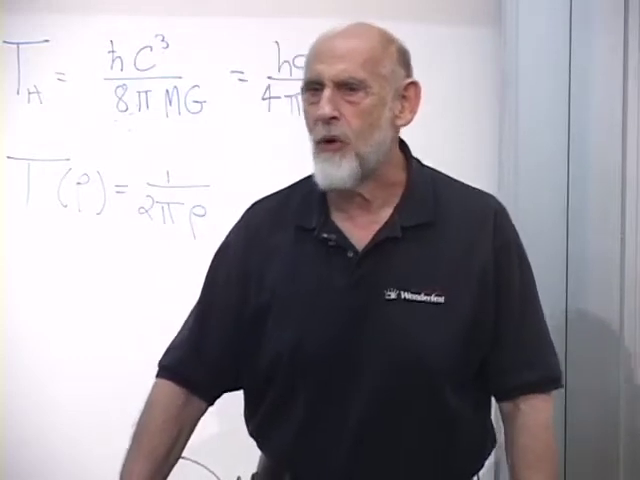
\includegraphics[width=0.72\textwidth]{lecture_05_figure_07.png}
\caption{渐近霍金温度与黑板上的视界附近局部温度\(T(\rho)=1/(2\pi\rho)\)。}
\lectureframe{01:02:40.000}
\end{figure}

一个用缆绳固定在\(\rho\)处的微小温度计，在被放下时会报告温度升高。维持在该静态大气中的原子会先被激发，然后电离，再解离；在更大的局部能量下，甚至原子核和强子也无法保持完整。让人脚朝下下降会得到令人难忘的诊断：热脚。

\emph{保持}一词至关重要。这种发散属于由加速保持静止的探测器。它描述的是相对于外部时间红移的热大气。自由下落的探测器遵循不同的轨迹，并且对于处于正则量子态中的足够大的黑洞，不必在视界处遇到发散的浴场。\editorialnote{这一区分将静态观察者看到的托尔曼温度和加速温度与自由下落观察者的正则局部体验区分开来。讲座有意将这种对比变成一个操作性问题，而不是仅靠术语来解决它。}

电离阈值使这一冲突变得具体。

\begin{classroomqa}
\audiencequestion{电离氢需要多少能量？\lecturetimestamp{01:06:53}}
\lecturerresponse{课堂上给出的是\(13\)电子伏特，正确地指出了\(13.6\,\mathrm{eV}\)基态电离能。随附的几千开尔文的估计太小，但论证只需要存在一个有限的阈值。}
\end{classroomqa}

确实，
\begin{equation}
\frac{13.6\,\mathrm{eV}}{k_B}\simeq1.58\times10^5\,\mathrm{K}.
\end{equation}
因此存在某个小的固有距离\(\rho_{\mathrm{ion}}\)，在该处静态温度达到电离尺度。静态外推表明，原子在那里——在视界之外——就应该已经电离了。相比之下，自由下落的原子预期不存在局域的墙，并且可以在有限的固有时间内穿过视界。外部观察者能否进行一项实验，在这两种描述之间做出判定？

\section{海森堡显微镜}

在把这个问题应用于黑洞之前，先回顾一下光子显微镜。要以分辨率\(\Delta x\)定位一个粒子，探测波长必须满足
\begin{equation}
\lambda\lesssim\Delta x.
\end{equation}
此时一个光子至少携带动量
\begin{equation}
p_\gamma\gtrsim\frac{\hbar}{\Delta x}.
\label{eq:l05-microscope}
\end{equation}
散射该光子会产生同量级的反冲。如果先测量位置，随即检查速度，那么第二次测量所看到的是已被第一次测量改变的状态。这个实验制造出了它本意要排除的条件。

\begin{figure}[htbp]
\centering
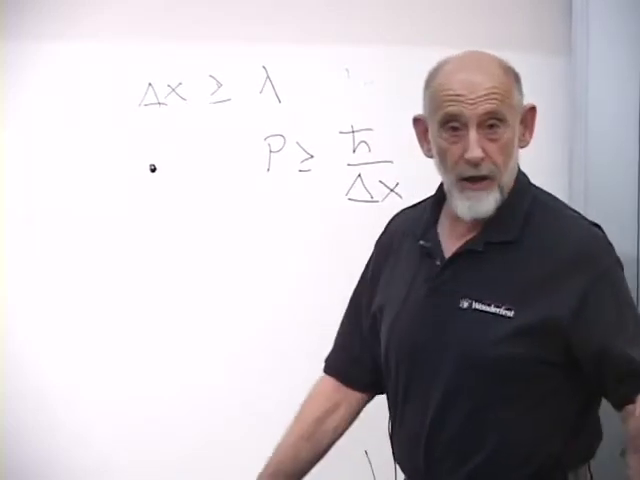
\includegraphics[width=0.70\textwidth]{lecture_05_figure_08.png}
\caption{显微镜估计\(\Delta x\gtrsim\lambda\)和\(p_\gamma\gtrsim\hbar/\Delta x\)。}
\lectureframe{01:11:50.000}
\end{figure}

这不仅仅是经典光学的局限。经典波可以被弄得任意弱；而量子力学要求在一次成功的探测事件中至少有一个量子。因此，提高空间分辨率就迫使产生有限的动量转移。

\section{近视界实验}

现在让一个原子从\(\rho_{\mathrm{ion}}\)处开始穿过这一层。相对于静态参考系，它以接近\(c\)的速度向内运动，因此在穿过视界之前可用的时间间隔为
\begin{equation}
\Delta\tau\sim\frac{\rho_{\mathrm{ion}}}{c}.
\label{eq:l05-fall-time}
\end{equation}
穿过之后，任何结果都无法传回外部。测量必须在这段短暂的时间间隔内区分完好的原子与电离的原子。

要在该层内分辨原子，需要
\begin{equation}
\lambda\lesssim\rho_{\mathrm{ion}}.
\end{equation}
因此探测能量受限于
\begin{equation}
E_\gamma=cp_\gamma
\gtrsim\frac{\hbar c}{\rho_{\mathrm{ion}}}.
\label{eq:l05-probe-energy}
\end{equation}
除因子\(2\pi\)外，这与方程~\eqref{eq:l05-local-temperature-si}是同一尺度：
\begin{equation}
E_\gamma\gtrsim2\pi k_B T_{\mathrm{loc}}(\rho_{\mathrm{ion}}).
\label{eq:l05-probe-temperature}
\end{equation}
能量足以分辨该事件的光子，其能量也足以电离该原子。

\begin{figure}[htbp]
\centering
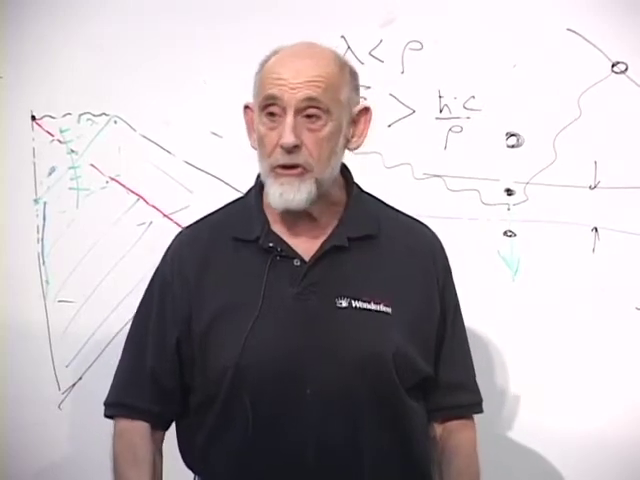
\includegraphics[width=0.72\textwidth]{lecture_05_figure_09.png}
\caption{黑板上的近视界估计：\(\lambda<\rho\)迫使局域探测能量达到\(\hbar c/\rho\)量级。}
\lectureframe{01:18:30.000}
\end{figure}

\begin{classroomqa}
\audiencequestion{那个高能光子在原子自身的自由下落参考系中也会电离该原子吗？\lecturetimestamp{01:19:07}}
\lecturerresponse{会。原子被一个真实的能量量子击中，并在其自身的局域参考系中反冲或电离。测量所揭示的并不是不受干扰的下落；它用受扰的下落取代了不受扰的下落。}
\end{classroomqa}

\begin{classroomqa}
\audiencequestion{如果原子只是下落，而没有人进行这个实验呢？\lecturetimestamp{01:19:39}}
\lecturerresponse{那么这种特定的扰动就不存在。如果外部观察者确实进行了高分辨率实验，原子就有麻烦了。这个论证关心的是从外部能够验证什么，而不是证明一个未被测量的下落者会被烧毁。}
\end{classroomqa}

\subsection{温度计或发射器能做得更好吗？}

移动仪器并不能消除信息问题。

\begin{classroomqa}
\audiencequestion{能否在更远处测量、推断梯度，或者让一个自由下落的温度计记录温度并在以后取回？\lecturetimestamp{01:19:51}}
\lecturerresponse{要获知近视界的记录，必须有某物与温度计相互作用，并以量子的形式把信息送回来。让温度计掉头需要剧烈的加速，而远程读取它则需要发射或散射。无论哪条途径，都会改变那个本应被检验其未受扰历史的物理系统。}
\end{classroomqa}

\begin{classroomqa}
\audiencequestion{小分辨率所需的高探测能量，与把反射观测从近视界区域送出去，是同一个困难吗？\lecturetimestamp{01:21:51}}
\lecturerresponse{它们是同一个红移尺度的两面。光子在最终到达无穷远时可以能量很低，因为它爬出来时损失了能量，但在它分辨原子的地方，它必须具有很高的局域频率。}
\end{classroomqa}

\editorialnote{仅仅为了逃逸，在视界外侧不远处发射的光子并不需要具有很大的能量。这里决定性的要求是，它要在\(\rho\)量级的固有时间和距离内编码该事件；于是引力红移把那个很大的局域频率与一个小得多的渐近频率联系起来。}

\begin{classroomqa}
\audiencequestion{物体能否自己发出信息，而不是被外部光子击中？\lecturetimestamp{01:22:51}}
\lecturerresponse{可以，但局域发射仍然需要足够的带宽，以辨认在短促时间间隔内发生了什么。发射还会给物体带来反冲。用发射器取代反射光，并不会产生无需代价的记录。}
\end{classroomqa}

\begin{classroomqa}
\audiencequestion{下落的原子有一个优先方向。它那有方向的动能被称为温度吗？\lecturetimestamp{01:23:10}}
\lecturerresponse{不是。扔出一个棒球并不会使棒球变热。整体下落能量与热骚动是不同的。论证中的温度属于周围静态辐射大气，而不属于原子的质心运动。}
\end{classroomqa}

\begin{classroomqa}
\audiencequestion{共同下落的实验室能否用磁场来检验原子是否被电离？\lecturetimestamp{01:23:50}}
\lecturerresponse{实验室可以进行局域检验。困难在于在穿越之前把结果传回外部。这种通信同样需要相互作用以及具有必要局域分辨率的出射量子。}
\end{classroomqa}

\begin{classroomqa}
\audiencequestion{如果温度计内置发射器，它会不会需要如此多的局域能量，以致摧毁仪器？\lecturetimestamp{01:24:57}}
\lecturerresponse{这就是同一障碍的工程形式。在足够靠近视界处，相关局域尺度上所需的信号能量与被检验的热尺度相当。}
\end{classroomqa}

\begin{classroomqa}
\audiencequestion{高温区域是否薄得没有时间从容进行测量？\lecturetimestamp{01:25:15}}
\lecturerresponse{正是如此。其固有厚度为\(\rho\)量级，穿越时间为\(\rho/c\)量级。人们可以把这一限制描述为空间分辨率或时间带宽；无论哪种描述，都要求高的局域动量或能量。}
\end{classroomqa}

相应的时间-带宽估计为
\begin{equation}
\Delta E\,\Delta\tau\gtrsim\hbar.
\end{equation}
这里应把它读作傅里叶分辨率或操作分辨率界限，而不是读作与\(\Delta x\,\Delta p\geq\hbar/2\)地位相同的算符不确定性关系。讲座只是启发式地援引时间-能量不确定性；由空间分辨率导出的方程~\eqref{eq:l05-probe-energy}才是论证中更坚实的部分。

\begin{classroomqa}
\audiencequestion{能否对许多原子使用较低能量、较低分辨率的探针，并以统计方式恢复答案？\lecturetimestamp{01:26:26}}
\lecturerresponse{这是一个合理的问题，课堂上对此保持开放。每个原子只提供一次通过，而任何被恢复的信号仍必须携带足够信息，以辨认短促的近视界事件。讲座诉诸不确定性原理，但并未给出完整的统计不可行性证明。}
\end{classroomqa}

\enlargethispage{2\baselineskip}
\section{已经确立与尚未确立的内容}

该论证并不预言自由下落者必定感受到发散的静态温度。

\begin{classroomqa}
\audiencequestion{我们是在说，我们可以预言下落者不会感受到温度吗？\lecturetimestamp{01:27:38}}
\lecturerresponse{不是。结论更狭窄：一个旨在确认原子未经历高温扰动的外部实验，会造成同一尺度的扰动。这就是这一操作分析所确立的全部内容。}
\end{classroomqa}

因此，结论不是防火墙定理，也不是下落者被烧毁的证明，更不是什么都不会发生的证明。它是对外部验证的限制：\emph{分辨未受扰动的近视界事件，需要一个会扰动它的探针}。
如果进行该实验，其量子就会产生它本要检验的效应。如果不进行该实验，仅凭这一论证并不能指定任何额外的实验上可及的事实。与双缝实验的类比是有意为之：在没有路径测量的情况下追问走了哪条缝，以及在没有相互作用的情况下追问外部装置能证实什么，都是在所提议的证据无法获得之处试图附加一个操作答案。
